In Fig. 1 and Fig. 2 we compare the pair correlation functions g(r) calculated with noisy forces and those evaluated with the standard approach. In Fig. 1 we show the pair correlation functions g(r) calculated with noisy forces generated from fixed point errors. In Fig. 2 we show the pair correlation functions g(r) calculated with noisy forces generated with floating point errors. We see from both Fig. 1 and Fig. 2, that the results are in agreement with our reference calculations and the use of noisy forces does not degrade the local structure and dynamics of the standard system. 

\begin{figure}[h!]%[!htpb,floatfix]
\begin{center}
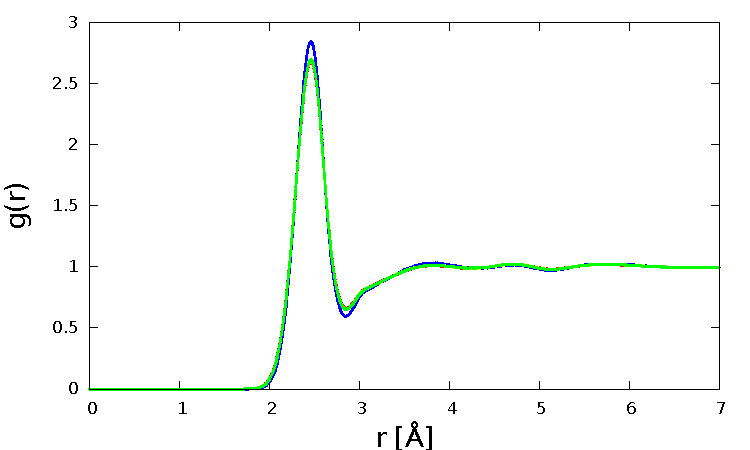
\includegraphics[width=0.475\textwidth]
{figures/fixedpoint.pdf}
\end{center}
\caption{\label{Fig1}
Pair correlation function for (a) liquid silicon (3000~K) in red and (b) liquid silicon (3000~K) with noisy forces introduced by fixed point errors corresponding to the values \(\left ( c.10^{-1 }\right ) \)(blue), \(\left ( c.10^{-2 }\right ) \)(yellow) and \(\left ( c.10^{-3 } \right ) \)(green).
} \end{figure}

\begin{figure}[h!]%[!htpb,floatfix]
\begin{center}
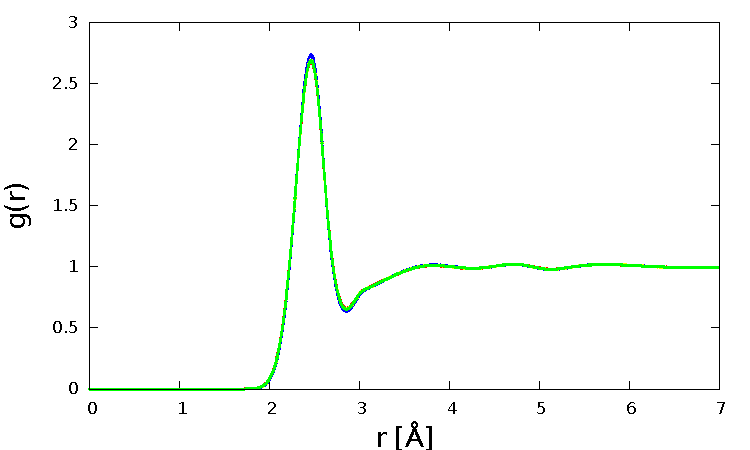
\includegraphics[width=0.475\textwidth]
{figures/floatingpoint.pdf}
\end{center}
\caption{\label{Fig2}
Pair correlation function for (a) liquid silicon (3000~K) in red and (b) liquid silicon (3000~K) with noisy forces introduced by floating point errors corresponding to the values \(c.10^{-(\alpha)}\)(blue), \(c.10^{-(\alpha+1)}\)(yellow) and \(c.10^{-(\alpha+2)}\)(green).
} \end{figure}

\begin{figure}[h!]%[!htpb,floatfix]
\begin{center}
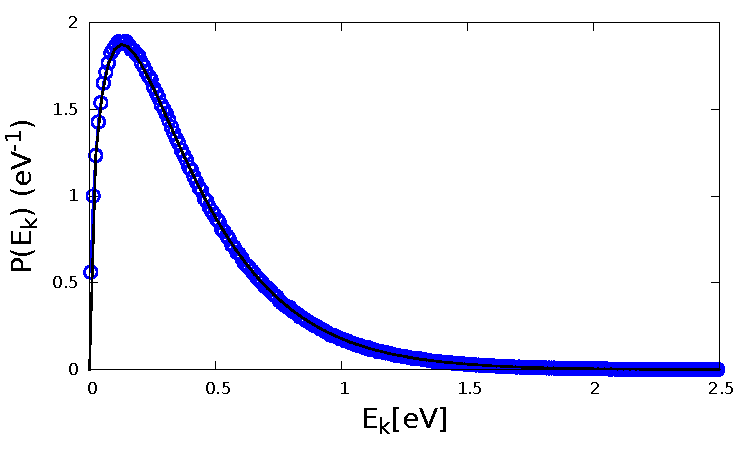
\includegraphics[width=0.475\textwidth]
{figures/maxwelldistribution.pdf}
\end{center}
\caption{\label{Fig3}
Statistical properties in a 1000 atoms liquid Si simulation at 3000~K. (a) The ionic kinetic energy distributions (line) is compared with the exact Maxwell distribution (circles).
} \end{figure}

In Fig. 3, the ionic kinetic energy distribution calculated with noisy forces is compared with the exact Maxwell distribution line and it can be seen that not only the average energy is correct but also its fluctuations follow the Maxwell distribution. 

\begin{figure}[h!]%[!htpb,floatfix]
\begin{center}
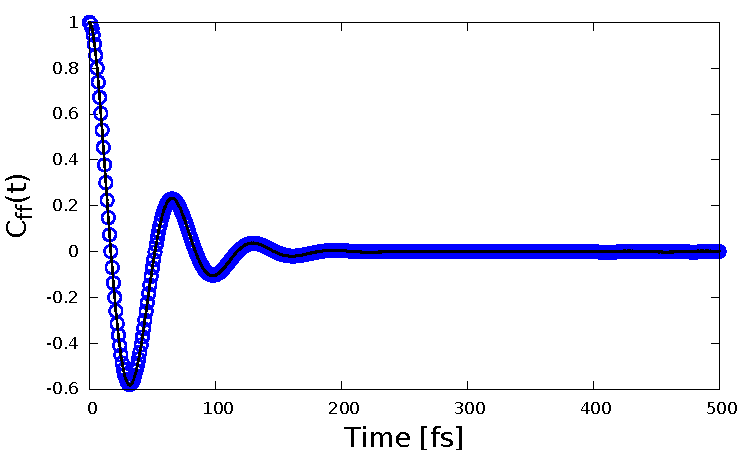
\includegraphics[width=0.475\textwidth]
{figures/force_autocorrelation.pdf}
\end{center}
\caption{\label{Fig4}
The Autocorrelation of the noisy force \(
\left \langle \textbf{F}_{I}^{FPGA}\left ( 0 \right ) \textbf{F}_{I}^{FPGA}\left ( t \right )\right \rangle \)(line) is compared with the autocorrelation of the exact force \( \left \langle \textbf{F}_{I}\left ( 0 \right ) \textbf{F}_{I}\left ( t \right )\right \rangle \)(circles). 
} \end{figure}

The autocorrelation of the noisy force is expanded by the following equation, 

\begin{subequations}
\begin{equation}
\begin{split}
\left \langle \textbf{F}_{I}^{FPGA}\left ( 0 \right )\textbf{F}_{I}^{FPGA}\left ( t \right )\right \rangle = \linebreak \\ \left \langle \left ( \textbf{F}_{I}\left ( 0 \right ) + \mathbf{\Xi } _{I}^{N}\left(0 \right )\right) \left( \textbf{F}_{I}\left ( t \right )+\mathbf{\Xi } _{I}^{N}\left ( t \right )\right) \right \rangle
\end{split}
\end{equation}

\begin{equation}\label{eq:1}
\begin{split}
\left \langle \textbf{F}_{I}^{FPGA}\left ( 0 \right )\textbf{F}_{I}^{FPGA}\left ( t \right )\right \rangle = \left \langle \textbf{F}_{I}\left ( 0 \right ) \textbf{F}_{I}\left ( t \right )\right \rangle + \linebreak \\\left \langle \textbf{F}_{I}\left ( 0 \right ) \mathbf{\Xi } _{I}^{N}\left(t \right )\right \rangle +  \left \langle \textbf{F}_{I}\left ( t \right ) \mathbf{\Xi } _{I}^{N}\left(0 \right )\right \rangle + \left \langle \mathbf{\Xi } _{I}^{N}\left(0 \right ) \mathbf{\Xi } _{I}^{N}\left(t \right )\right \rangle
\end{split}
\end{equation}
\end{subequations}

In Eq. (\ref{eq:1}), the cross correlation terms between exact force and the additive white noise becomes zero, thereby giving us an equation where the autocorrelation of noisy force is equal to the autocorrelation of the exact force. From Fig. 4, we prove this behavior where the autocorrelation of the noisy force is compared with the autocorrelation of the exact force. 

If the random value that was used to generate the computational error is chosen in the range [0,1] instead of [-0.5,0.5], we encounter a phenomenon called "Flying Ice Cube" \cite{flyingIceCube} during our MD simulations.  
